\documentclass[12pt]{article}
\usepackage[margin=1.2in]{geometry}
\usepackage[all]{nowidow}
\usepackage[hyperfigures=true, hidelinks, pdfhighlight=/N]{hyperref}
\usepackage{graphicx,amsmath,physics,tabto,float,amssymb,pgfplots,verbatim,tcolorbox}
\usepackage{listings,xcolor,siunitx,subfig,keyval2e,caption}
\definecolor{stringcolor}{HTML}{C792EA}
\definecolor{codeblue}{HTML}{2162DB}
\definecolor{commentcolor}{HTML}{4A6E46}
\lstdefinestyle{appendix}{
    basicstyle=\ttfamily\footnotesize,commentstyle=\color{commentcolor},keywordstyle=\color{codeblue},
    stringstyle=\color{stringcolor},showstringspaces=false,numbers=left,upquote=true,captionpos=t,
    abovecaptionskip=12pt,belowcaptionskip=12pt,language=Python,breaklines=true,frame=single}
\lstdefinestyle{inline}{
    basicstyle=\ttfamily\footnotesize,commentstyle=\color{commentcolor},keywordstyle=\color{codeblue},
    stringstyle=\color{stringcolor},showstringspaces=false,numbers=left,upquote=true,frame=tb,
    captionpos=b,language=Python}
\renewcommand{\lstlistingname}{Appendix}
\pgfplotsset{compat=1.17}

\title{Integrating Equations of Motion: Orbits}
\date{\textbf{6 June 2020}}
\author{}

\begin{document}

    \maketitle
    \begin{center}
    \textbf{\large{PHY2004W}}
    \textbf{\large{KDSMIL001}}
    \end{center}
    \tableofcontents
    
    \section{Introduction}
    In this Assignment, we aim to simulate the Two- and Three-Body problems using vPython. These problems 
    involve analysing the movement of 2 and 3 bodies interacting with each other, in this case at least, 
    by the force of gravity. These are hard, in some cases impossible, to solve analytically so we use 
    numerical methods to try and get an idea of the general qualities of these systems. Note that this 
    does not give us an exact solution. In many cases our solution will diverge from the actual solution 
    as the system is intrinsically chaotic, but there are a few tricks we can employ to reduce this effect.

    \section{Activity}
    \begin{enumerate}
        \item \textbf{The Two-Body Problem} \newline
        Before we get to our methods of numerical integration, we must first establish the theory behind 
        the steps we will take. We will be using Newton's equation for gravitational force between two 
        objects:
        \begin{equation}
            \vec{F}_{12} = -Gm_1m_2\frac{\vec{r}_1-\vec{r}_2}{|\vec{r}_1-\vec{r}_2|^3}
        \end{equation}
        where $\vec{F}_{12}$ is the force on mass 1 due to mass 2, $m$ is the mass of an object, and 
        $\vec{r}$ is the position vector of an object. \newline
        Now we can move on to how we will simulate this system. We will use the Symplectic Euler Method, 
        which involves using the force from the next time step in order to calculate the momentum and 
        position for that time step. This is obviously a discrete method of integration and is prone to 
        deviations from the actual value. This is the divergence we spoke about above. One of the tricks we 
        can use to reduce this effect is, apart from using the Symplectic Euler Method, decreasing the size 
        of our time step. \newline
        To start off, we'll run with the most simple initial conditions, even considering one of the masses 
        to be much larger than the other (think of the Sun and the Earth). We mean this as the one mass 
        doesn't move. For the sake of simplicity and size, their masses in the simulation are the same but 
        the Star is fixed in place.

        \begin{figure}[h]
            \begin{center}
               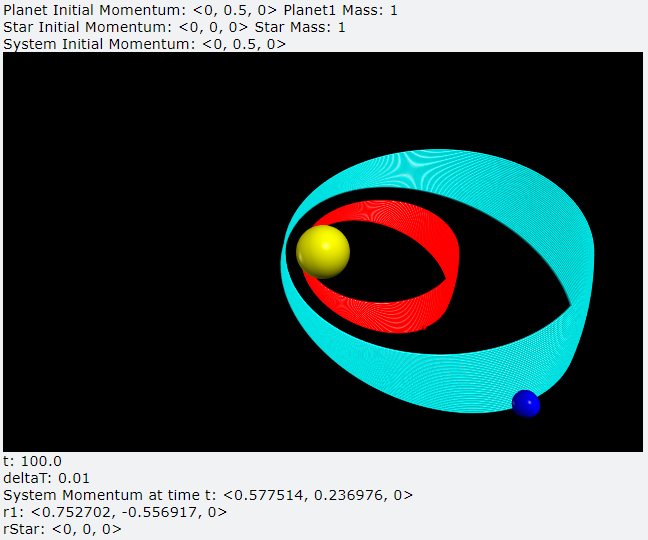
\includegraphics[scale=.5]{TwoBody1.png}
               \caption{A Small Time Step}
               \label{fig:TwoBody1}
            \end{center}
        \end{figure}
        \noindent
        The red sphere and trail is the position of the Centre of Mass of the system. As you can 
        see, in \autoref{fig:TwoBody1} the ``Earth's'' orbit precesses. This happens because, once the 
        system has finished an orbit, due to error in the approximation, the planet is not at exactly 
        the same place as it was when it started. This continues every orbit.If we decrease the time 
        step, we can see that that doesn't happen as much. 

        \begin{figure}[h]
            \begin{center}
               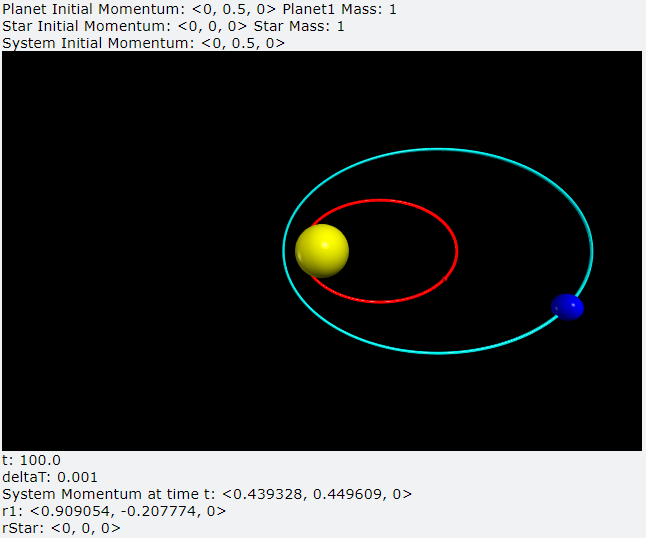
\includegraphics[scale=.5]{TwoBody2.png}
               \caption{A Smaller Time Step}
               \label{fig:TwoBody2}
            \end{center}
        \end{figure}
        \noindent
        Clearly, \autoref{fig:TwoBody2} is much more accurate. This makes sense as our method approximates the 
        solution at each step as a straight line. With a larger time step, there's more room at each step 
        for the approximation to diverge from the actual solution. This shortcoming of our method becomes 
        even more apparent when we consider the system at high velocities. We can try to predict what will 
        happen: \newline
        Our method approximates the solution as a straight line. At relatively low velocities, this means 
        that at each time step the distance covered is quite small, meaning the approximation is close 
        to the actual solution as there isn't much that can go wrong. At higher velocities, the distance 
        covered is much higher, meaning that our straight line approximation can diverge more over the same 
        time step than for smaller distances. We can check this by running 2 identical simulations, apart 
        from the starting momenta. Firstly we'll try a mildly eccentric orbit in \autoref{fig:TwoBody3}

        \begin{figure}[H]
            \begin{center}
               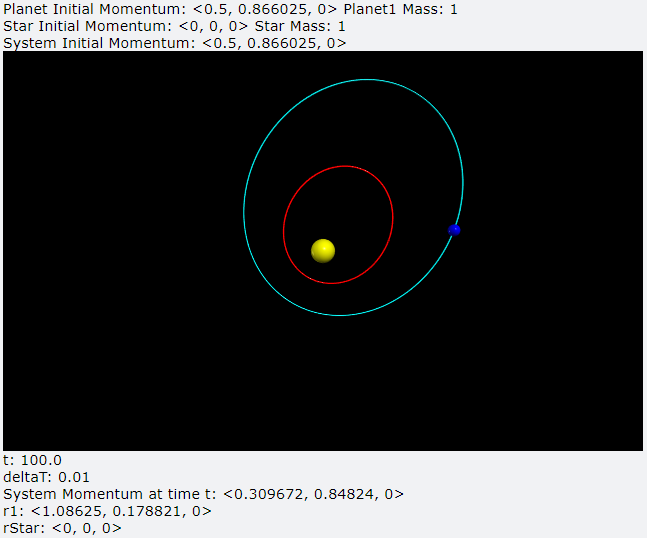
\includegraphics[scale=.5]{TwoBody3.png}
               \caption{A Mildly Eccentric Orbit}
               \label{fig:TwoBody3}
            \end{center}
        \end{figure}
        \noindent
        We can see that this is a reasonable system. It doesn't precess, at least not noticeably, even after 
        a long time. It even conserves momentum quite well. Compare that to \autoref{fig:TwoBody4}.

        \begin{figure}[H]
            \begin{center}
               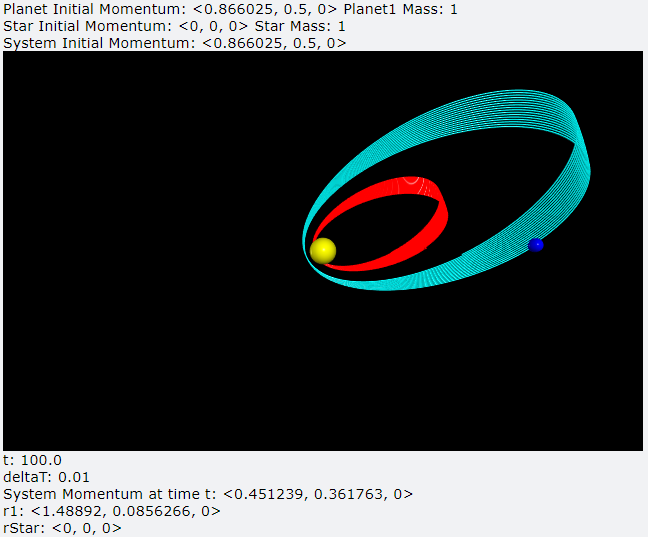
\includegraphics[scale=.5]{TwoBody4.png}
               \caption{A Wildly Eccentric Orbit}
               \label{fig:TwoBody4}
            \end{center}
        \end{figure}
        \noindent
        After the same amount of time, the system has clearly precessed quite a bit and the total momentum 
        at the end is completely different to the starting momentum in terms of magnitude. So we now know 
        that our method has some limitations. Decreasing the time step will increase runtime but greatly 
        increase accuracy. We must just consider these facts as we move forward. \newline
        \newline
        Next up, we can see what would happen if, instead of employing a Symplectic Euler Method where we 
        use the following step's momentum to calculate that step's change in position, we first update the 
        position and \emph{then} update the momentum. This is the plain old Euler's Method and it yields 
        some interesting results to think about (\autoref{fig:TwoBody5}).

        \begin{figure}[h]
            \begin{center}
               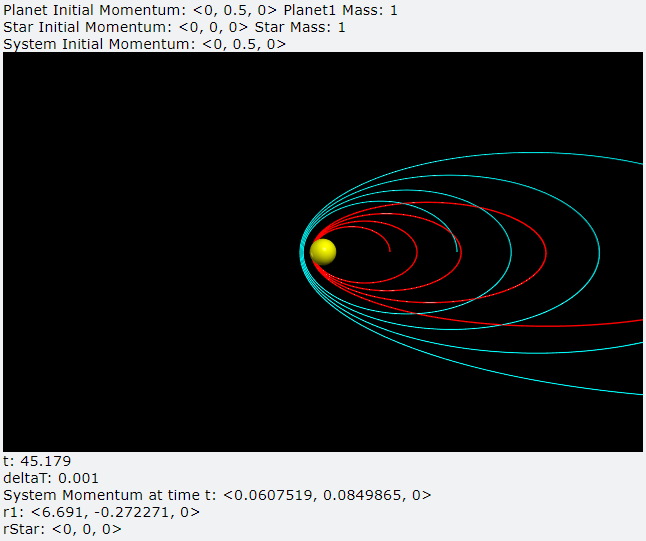
\includegraphics[scale=.5]{TwoBody5.png}
               \caption{A Smaller Time Step with Euler's Method}
               \label{fig:TwoBody5}
            \end{center}
        \end{figure}
        \noindent
        Clearly the program is overestimating the momentum at each time step, leading to growth of orbits. 
        \newline
        Next up, we investigate a slight modification to the Potential Energy. It is known that gravitational 
        force is the gradient of potential in the form
        \begin{equation}
            \vec{F}_G = -\grad U = \grad Gm_1m_2\frac{1}{|\vec{r}_2-\vec{r}_1|}
            \label{eqn:ForceGradU}
        \end{equation}
        If we change this potential to be in the form 
        \begin{equation*}
            U \propto -\frac{1}{r^{1+\epsilon}}
        \end{equation*}
        where $\epsilon \in [0.1, 0.3]$, we will find the force to be 
        \begin{equation}
                \vec{F}_G = -Gm_1m_2\frac{\epsilon+1}{|r_2-r_1|^{\epsilon+3}}\vec{r}
                \label{eqn:AdjustedPotentialForce}
        \end{equation}
        Implementing this equation into our program, we get the following results:
        \begin{figure}[H]
            \begin{center}
               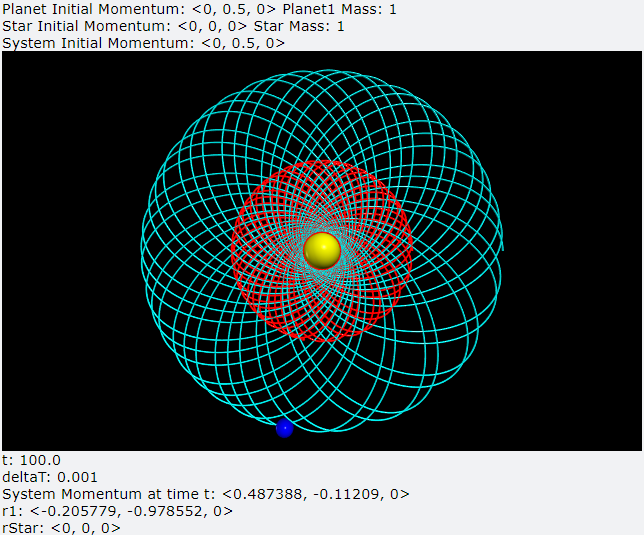
\includegraphics[scale=.5]{TwoBody6.png}
               \caption{Adjusted Potential with $\epsilon = 0.1$}
               \label{fig:TwoBody6}
            \end{center}
        \end{figure}
        \begin{figure}[H]
            \begin{center}
               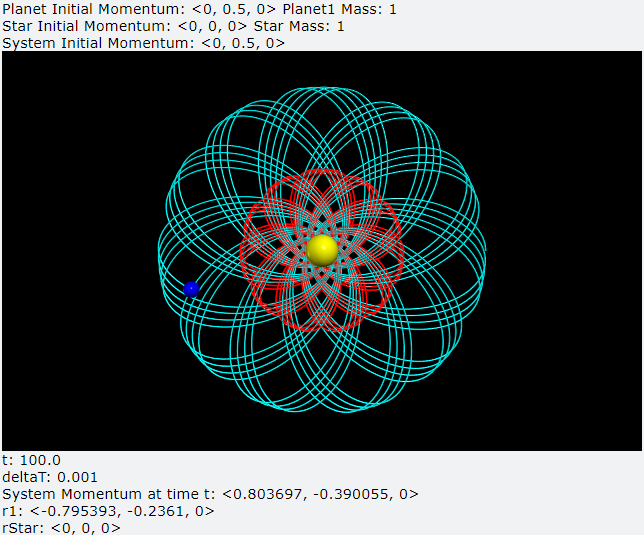
\includegraphics[scale=.5]{TwoBody7.png}
               \caption{Adjusted Potential with $\epsilon = 0.3$}
               \label{fig:TwoBody7}
            \end{center}
        \end{figure}
        \noindent
        It seems that, predictably, with higher values of $\epsilon$, the magnitude of the force increases. 
        We expect this as the denominator from \autoref{eqn:AdjustedPotentialForce} grows faster as 
        $\epsilon$ grows, so the force should grow too. The precession would come from the $\epsilon+1$ 
        term.        
        \newline
        Now we can finally get to the interesting stuff: Two bodies of similar mass orbiting each other. 
        We shall return to the Symplectic Euler Method, with the potential as it should be. 
        It's relatively simple to convert the program as we are already calculating the force between the 
        bodies, so we need only reverse the direction to find the force on the star. If we let the 
        star feel the force between the two bodies, with the same initial conditions as in 
        \autoref{fig:TwoBody2}, we get \autoref{fig:TwoBody8}. 
        \begin{figure}[h]
            \begin{center}
               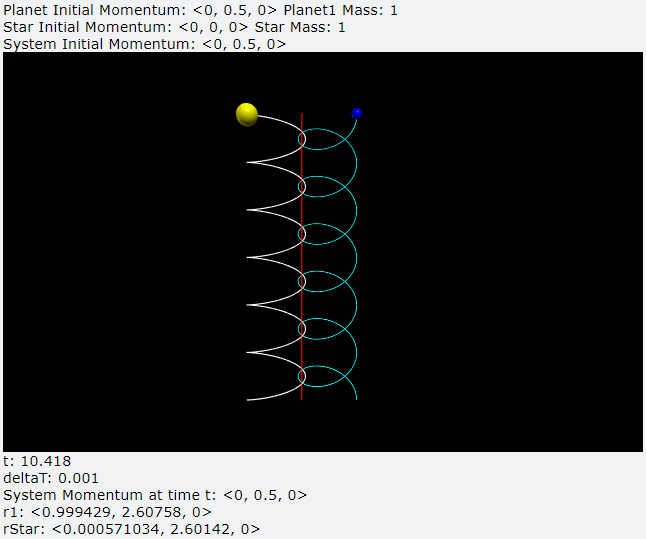
\includegraphics[scale=.5]{TwoBody8}
               \caption{Two-Body System with Star able to move}
               \label{fig:TwoBody8}
            \end{center}
        \end{figure}
        \newline
        This seems to be stable, and is a reasonable system, but the system drifts as the starting momentum 
        is non-zero. This can be fixed in 2 ways. The quick fix is to have starting conditions that give us 
        a total momentum of 0. This is trivial and not really helpful in the grand scheme of things, so we 
        can try another fix. If we adjust the coordinates as below we will always have the centre of mass 
        stay still in our window. This is because it automatically adjusts the momenta to have a total 
        momentum of 0.
        \lstinputlisting[title=Adjustment of Coordinates, style=inline, linerange=12-15, firstnumber=12]{CP6_TwoBody.py}
        This method with similar conditions gives us \autoref{fig:TwoBody9}
        \begin{figure}[H]
            \begin{center}
               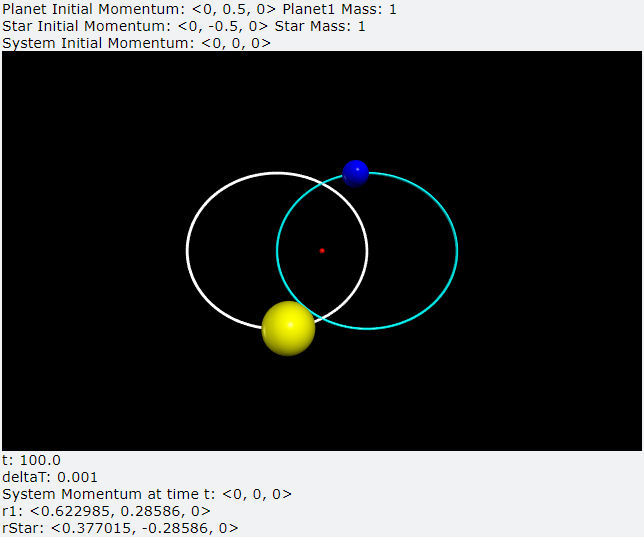
\includegraphics[scale=.5]{TwoBody9.png}
               \caption{Two-Body System with Adjusted Coordinates}
               \label{fig:TwoBody9}
            \end{center}
        \end{figure}
        \noindent
        This is a very stable system. Actually, most initial conditions for the Two-Body problem result in 
        stable and periodic motion. It's also clear that this system now perfectly conserves momentum, which 
        is a comforting side effect.
        \newpage


    \end{enumerate}


\end{document}